\oldpage{404}

\begin{center}
\begin{tabbing}
  \prescription. \= Prussiate of Iron,  \\
    \> Hydrastin, āā \dram{} ss.
\end{tabbing}
\end{center}
Mix.\quad{}Make 15 powders, two to be taken a day. The patient felt
well and returned home, and now nearly one year has remained well as
usual.

\begin{figure}[H]
  \centering
  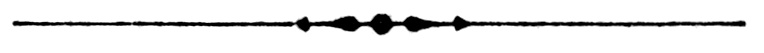
\includegraphics{pages/illustrations/arrow_bullet_divider.jpg}
\end{figure}

\section*{What Influence has the Moon Upon Disease?}

\byline*{\ProperName{Comely Jessup},\ \md}

\SectionStartWords{I wish} to ask your opinion and procure, if possible, the result of the
observations of your readers, relating to the influence (if such influence
exist), exerted by the moon upon disease. I have been of the number
who look upon the lunar influences except such as may be attributed to
the known laws of gravitation as entirely fabulous, but several instances
occurring within the sphere of my observation, which have indicated
the existence of some hidden agency, a few of which have been distinctly
marked, have awakened a desire to see the matter thoroughly
investigated and the truth or falsity of lunar influence fairly demonstrated.
The following are a few of the more marked instances of apparent lunar
periodicity which have fallen under my observation.

\textsc{Case 1.} Mr.~C., aged perhaps 45, has been subject to epilepsy for
the last three years. About the time of the change and full of the
moon he will have from three or four to eight or ten convulsions. At
other times he is free from them, except occasionally about the time of
the first and last quarter.

\textsc{Case 2.} T.~I., aged 72, was attacked some four years since with malignant
erysipelas, accompanied at first with paralytic symptoms,
which, together with a severe attack of ``Doctors,''---though he survived
them all---left him in a condition from which he has never recovered
and never will. The most prominent features in his case now
are pain in the back and head, which is remittent in its character,
being most severe in the early part of the day; nervousness, constant
trembling of the hands, or rather the peculiar shaking characteristic of
paralysis, to the extent that he can with difficulty feed himself; and
occasional attacks of general weakness and disposition to syncope.
These \typo{symptoms}{symptems} are all much aggravated at the time of the moon's
changes.

\textsc{Case 3}. A.~E.~S., aged 5; troubled with ascaris vermicularis at
the time of the new and full moon, which were during the intervening\endinput
